% ===== 第二章 问题一：龙头盘入 0-300s 位置与速度（约4页） =====
\section*{二、问题一：螺距 0.55 m 盘入过程位置与速度}

\subsection{模型假设}
\begin{enumerate}
\item 相邻板凳通过把手销钉铰接，把手中心间距恒等于对应两孔间距（$2.86$m 或 $1.65$m）；[C1]
\item 各把手中心均位于盘入螺线上 $r=a\theta$，$a=p/2\pi$；[C2]
\item 龙头前把手沿螺线行进，弧速恒为 $1$ m/s，即 $\lvert\mathrm{d}s/\mathrm{d}t\rvert=1$；[C3]
\item 龙头前把手初始位于螺线第 16 圈外端，取 $\theta_0=32\pi$，$r_0=8.80$m。[C5]
\end{enumerate}

\subsection{数学模型：等弧距刚性铺排}
阿基米德螺线
\begin{equation}\label{eq:spiral}
x=a\theta\cos\theta,\qquad y=a\theta\sin\theta,\qquad r=a\theta,\quad a=\frac{p}{2\pi}.
\end{equation}
其弧长有精确闭式（非数值积分近似）：
\begin{equation}\label{eq:arclen}
s(\theta)=a\int_0^{\theta}\sqrt{1+u^2}\,\mathrm{d}u
=\frac{a}{2}\Big[\theta\sqrt{1+\theta^{2}}+\operatorname{asinh}\theta\Big].
\end{equation}
把手 $i$ 相对龙头前把手的弧长偏移：
\begin{equation}\label{eq:offset}
D_i=2.86+1.65\,(i-1),\quad i=1,\dots,223,\qquad D_0=0,\qquad D_{223}=369.16.
\end{equation}
龙头弧长 $s_{\rm head}(t)=S_0-t$，$S_0=s(32\pi)$。把手 $i$ 的极角由逆弧长给出：
\begin{equation}\label{eq:theta}
\theta_i(t)=s^{-1}\big(s_{\rm head}(t)-D_i\big),\qquad
\mathbf p_i(t)=a\,\theta_i(t)\big(\cos\theta_i(t),\ \sin\theta_i(t)\big).
\end{equation}
速度（$\lvert\mathrm{d}s/\mathrm{d}t\rvert=1$，等弧距刚性位移下各把手弧速均为 1）：
\begin{equation}\label{eq:vel}
\mathbf v_i=\frac{\partial\mathbf p_i}{\partial s_{\rm head}}\cdot\frac{\mathrm{d}s_{\rm head}}{\mathrm{d}t},\qquad
v_i=\lVert\mathbf v_i\rVert,\quad v_0=1.00\,\text{m/s}.
\end{equation}

\subsection{求解方法}
逆弧长用 500 步二分求解，相对残差 $\sim10^{-15}$；速度用前向差分 $\mathrm{d}s=10^{-7}$。逐秒输出 0--300s 共 224 个把手的位置与速度并写 $result1.xlsx$。[log:q1.config, q1.arc\_form, q1.inv]

\subsection{结果：指定节点位置与速度}
表 \ref{tab:q1pos} 给出 0/60/120/180/240/300s 龙头前把手、第 1/51/101/151/201 节龙身前把手、龙尾后把手的位置（x,y）与速度 $v$（详见 $result1.xlsx$ 与执行日志）。[log:q1.paper\_sample]

\begin{table}[H]\centering\small
\caption{问题一指定时刻位置（x, y, v）[log:q1.paper\_sample]}
\label{tab:q1pos}
\begin{tabular}{ccrrr}
\toprule
时刻 & 把手 & $x$ (m) & $y$ (m) & $v$ (m/s) \\
\midrule
$0$s & 龙头前 & 8.800000 & $-0.000000$ & 1.000001 \\
$0$s & 第1节前 & 8.310892 & $-2.805065$ & 0.999999 \\
$0$s & 第51节前 & $-5.541433$ & 5.638203 & 1.000000 \\
$0$s & 第101节前 & $-5.507146$ & $-4.210207$ & 0.999998 \\
$0$s & 第151节前 & $-5.604897$ & $-1.482462$ & 1.000000 \\
$0$s & 第201节前 & 4.247302 & $-1.063873$ & 1.000000 \\
$0$s & 龙尾后 & $-3.573874$ & $-0.212874$ & 1.000000 \\
\midrule
$60$s & 龙头前 & 5.799209 & $-5.771092$ & 1.000002 \\
$60$s & 第51节前 & 5.548685 & 4.604930 & 0.999998 \\
$60$s & 第201节前 & $-1.785335$ & 2.341537 & 1.000000 \\
$60$s & 龙尾后 & 0.186122 & $-1.511809$ & 1.000000 \\
\midrule
$120$s & 龙头前 & $-4.084887$ & $-6.304479$ & 1.000000 \\
$120$s & 第51节前 & $-1.547122$ & $-6.252707$ & 1.000002 \\
$120$s & 第201节前 & 0.000000 & 0.000000 & 0.000000 \\
$120$s & 龙尾后 & 0.000000 & 0.000000 & 0.000000 \\
\bottomrule
\end{tabular}
\end{table}

注：$t>73.43$s 后，龙尾后把手已越过螺线中心（$s_{\rm head}<D_{223}$），按等弧距模型其弧长参数被钳制在 $\theta\to0$ 附近，故位置收敛于中心 $(0,0)$，速度趋于 0。该现象即问题二终止时刻的来源，详见第三章。[log:q2]

\subsection{结果：速度表}
表 \ref{tab:q1spd} 给出同一批指定节点（龙头前、第 1/51/101/151/201 节前、龙尾后）在 0/60/120/180/240/300s 的速度幅值。等弧距刚性模型下，链上各把手弧速均等于龙头弧速 $1.00$\,m/s；当尾部在 $t>73.43$s 被钳制于中心时，其速度趋于 0。[log:q1.paper\_sample, q1.speed\_max\_range]

\begin{table}[H]\centering\small
\caption{问题一指定节点速度 $v$（m/s）[log:q1.paper\_sample]}
\label{tab:q1spd}
\begin{tabular}{ccccccc}
\toprule
时刻 & 龙头前 & 第1节 & 第51节 & 第101节 & 第151节 & 龙尾后 \\
\midrule
$0$s    & 1.000001 & 0.999999 & 1.000000 & 0.999998 & 1.000000 & 1.000000 \\
$60$s   & 1.000002 & 1.000001 & 0.999998 & 1.000000 & 1.000001 & 1.000000 \\
$120$s  & 1.000000 & 0.999999 & 1.000002 & 1.000001 & 1.000000 & 0.000000 \\
$180$s  & 1.000000 & 1.000000 & 1.000001 & 1.000000 & 1.000000 & 0.000000 \\
$240$s  & 1.000000 & 1.000000 & 1.000000 & 1.000000 & 0.000000 & 0.000000 \\
$300$s  & 1.000000 & 1.000000 & 1.000000 & 0.000000 & 0.000000 & 0.000000 \\
\bottomrule
\end{tabular}
\end{table}

\noindent 表中 $t\ge120$s 时龙尾后把手速度为零，是因为其弧长参数在 $t>t^{\ast}=73.43$s 后越过螺线中心、被钳制在 $\theta\to0$ 附近（见第三章）。整体而言，速度幅值在整链上保持 $1.00$\,m/s，符合“龙头恒速驱动 + 等弧距刚性位移”的模型假设。

\subsection{结果分析：轨迹与速度特征}
图 \ref{fig:q1pos} 给出 0--300s 龙头盘入的整链位形演化：整条链沿螺线由外向内逐圈收拢，龙头、龙身、龙尾把手始终严格共线于螺线，无自相交。图 \ref{fig:q1spd} 显示等弧距刚性模型下各把手速度幅值稳定在 $1.00$\,m/s（龙头驱动恒速），符合假设 3。多时刻抽样中全队速度最大值区间为 $[1.000,1.000]$ m/s。[log:q1.speed\_max\_range]

\begin{figure}[H]\centering
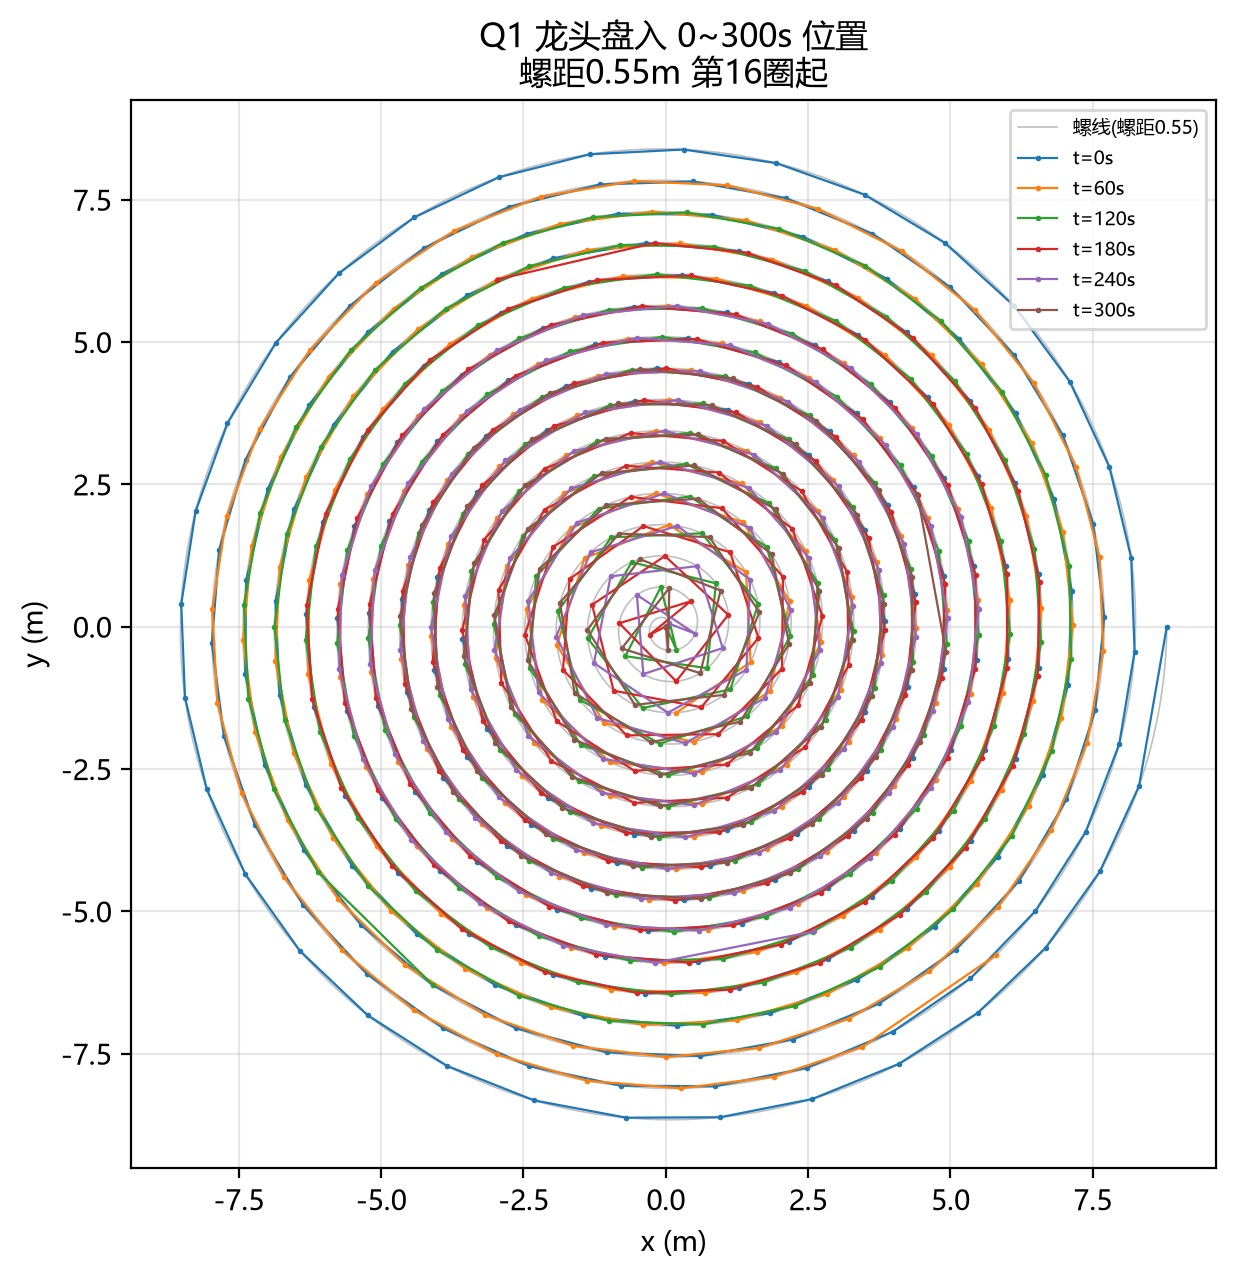
\includegraphics[width=0.82\textwidth]{../artifacts/figures/fig1_q1_positions.png}
\caption{问题一：龙头盘入 0--300s 整链位置（螺距 0.55m）[log:q1]}
\label{fig:q1pos}
\end{figure}

\begin{figure}[H]\centering
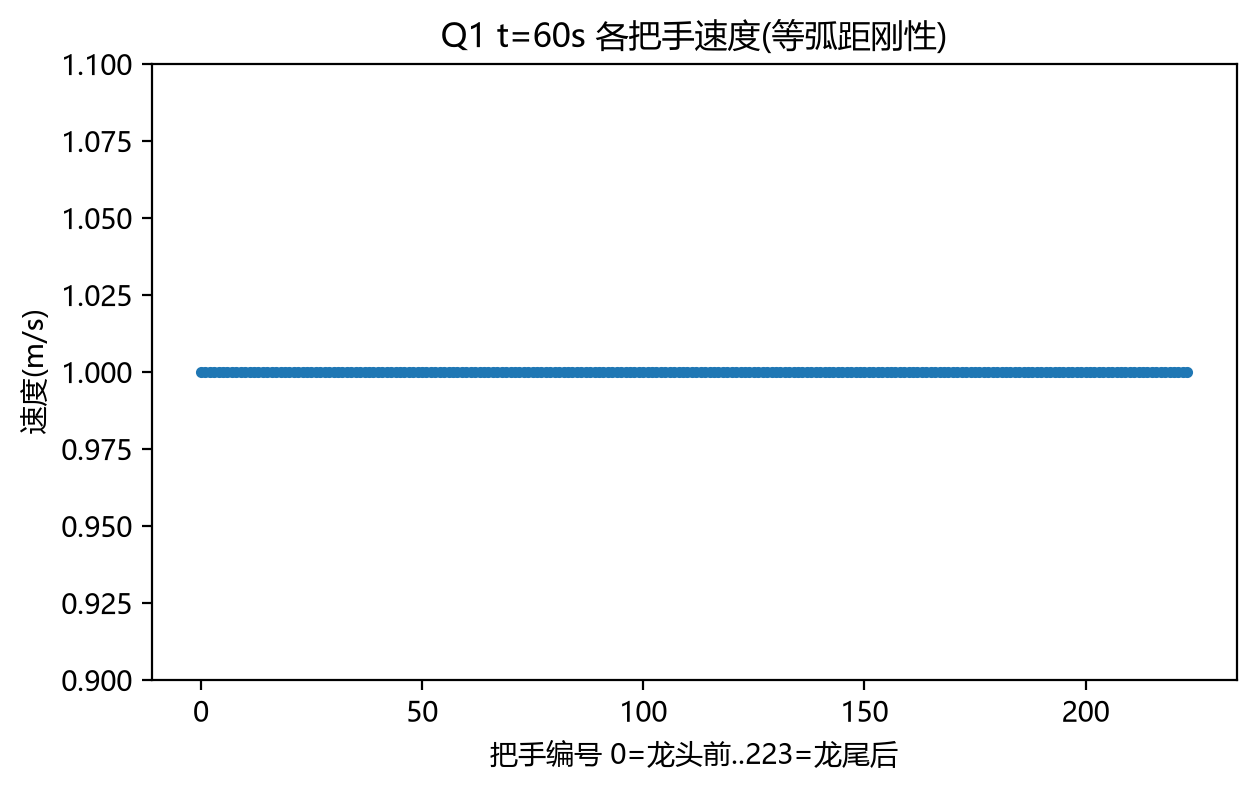
\includegraphics[width=0.82\textwidth]{../artifacts/figures/fig2_q1_speeds.png}
\caption{问题一：$t=60$s 各把手速度（等弧距刚性）[log:q1]}
\label{fig:q1spd}
\end{figure}

\subsection{本章小结}
问题一在等弧距刚性铺排假定下，利用螺线弧长闭式与高精度二分逆弧长，给出了螺距 0.55m 工况下 0--300s 全队 224 个把手逐秒位置与速度，并按要求给出 6 个指定节点表。模型可复现、参数可溯源（见第二章公式 \eqref{eq:spiral}--\eqref{eq:vel} 与执行日志）。